\documentclass[english]{article}
\usepackage[T1]{fontenc}
%\usepackage[latin9]{inputenc}
%\usepackage{geometry}
%\geometry{verbose,tmargin=1in,bmargin=1in,lmargin=1in,rmargin=1in}
\usepackage{amsmath}
\usepackage{amssymb}
\usepackage{setspace}
\usepackage[utf8]{inputenc}
\usepackage{graphicx}
\usepackage{float}
\usepackage{adjustbox}
\usepackage{gensymb}
\usepackage{amssymb}
\usepackage{array}
\usepackage{ragged2e}
\usepackage{lipsum}
\onehalfspacing
\usepackage{babel}
\usepackage{tikz}
\usepackage{ctable}
\usepackage{booktabs}
\usepackage{graphicx}
\usepackage{caption}
\usepackage{placeins}
\usepackage{todonotes}
\usepackage{subcaption}
\usepackage[font=footnotesize,labelformat=simple]{subcaption}
\usepackage[T1]{fontenc}
\usepackage{pdflscape}

\begin{document}


\title{How much can we characterize self-employed workers?}
\maketitle

\section{Shares}

\begin{figure}[H]
            \justifying
                \caption{Share of employers of a small firms: owner of a firm with growth potential}  
            \centerline{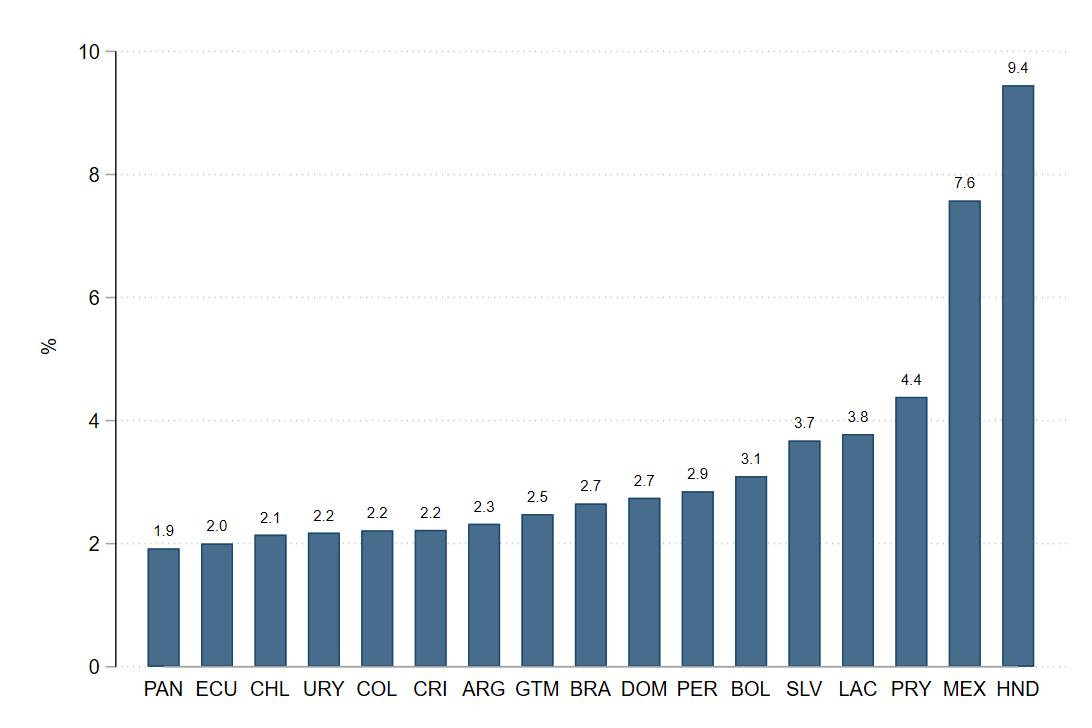
\includegraphics[scale=.3]{latex/figures/Self-employed/employer_growthfirms.png}}
                \label{fig:owner-}
                \footnotesize{Source: SEDLAC}
\end{figure}

\begin{figure}[H]
            \justifying
                \caption{Share of self-employed (independents and employers) who work in small firms}  
            \centerline{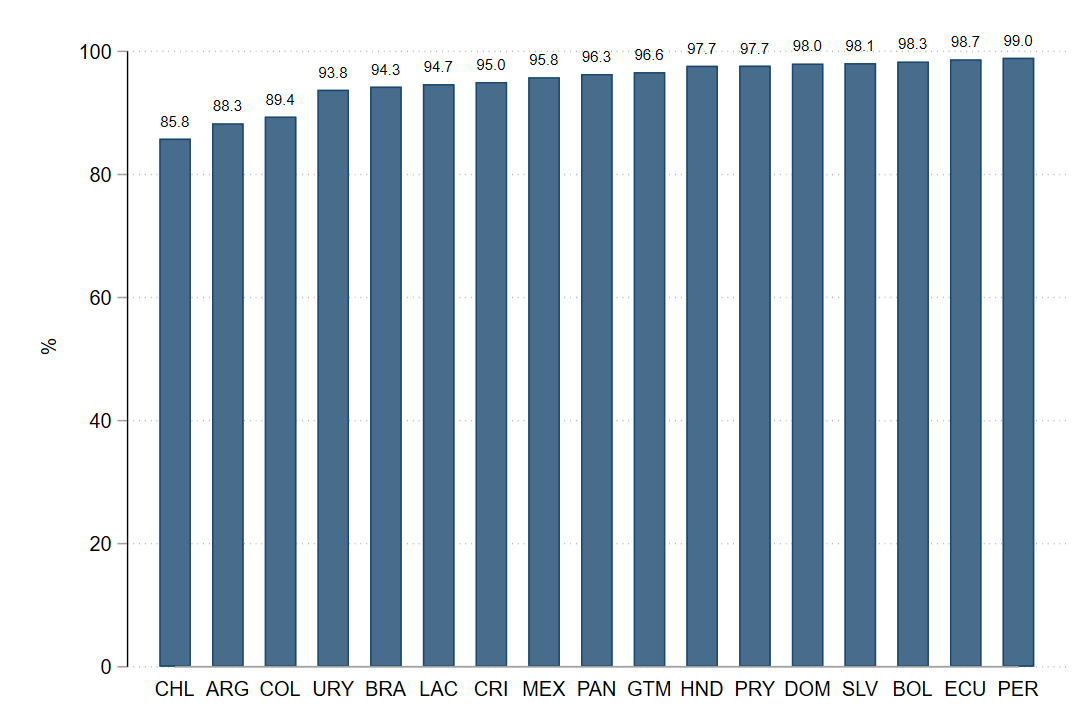
\includegraphics[scale=.3]{latex/figures/Self-employed/selfemployed_small.png}}
                \label{fig:owner-}
                \footnotesize{Source: SEDLAC}
\end{figure}

\begin{figure}[H]
            \justifying
                \caption{Share of self-employed (without employers): independent contractor}  
            \centerline{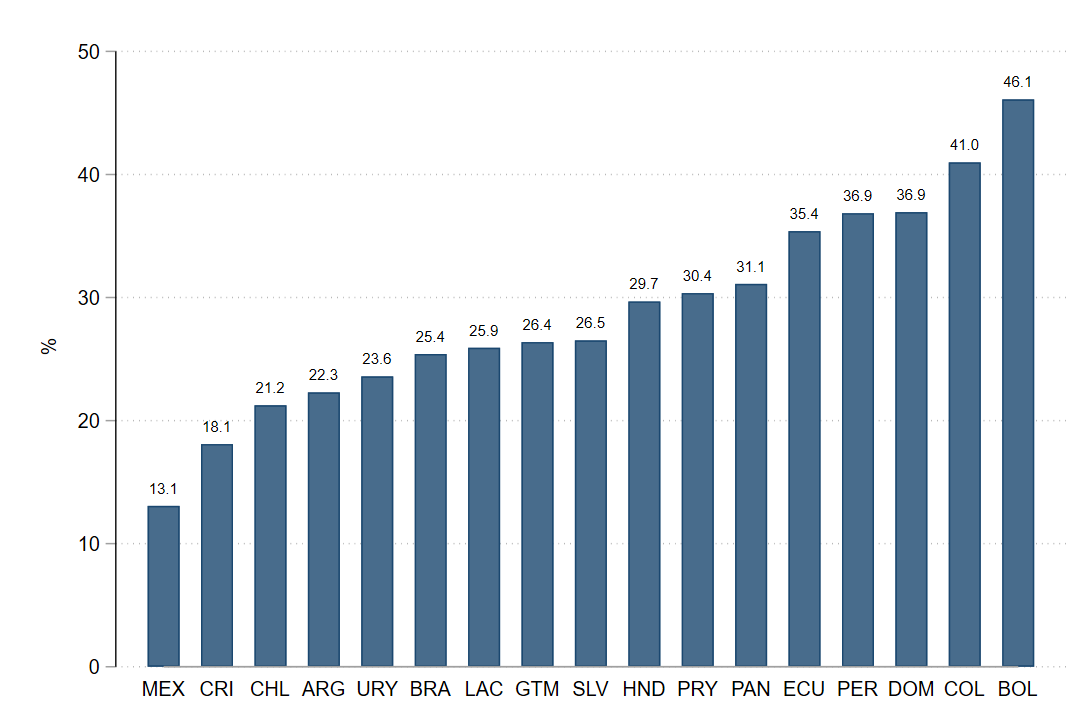
\includegraphics[scale=.3]{latex/figures/Self-employed/independent.png}}
                \label{fig:owner-}
                \footnotesize{Source: SEDLAC}
\end{figure}


\section{Contributes to SS}

\begin{figure}[H]
            \justifying
                \caption{Share of employers of small firms who does not contributes to SS}  
            \centerline{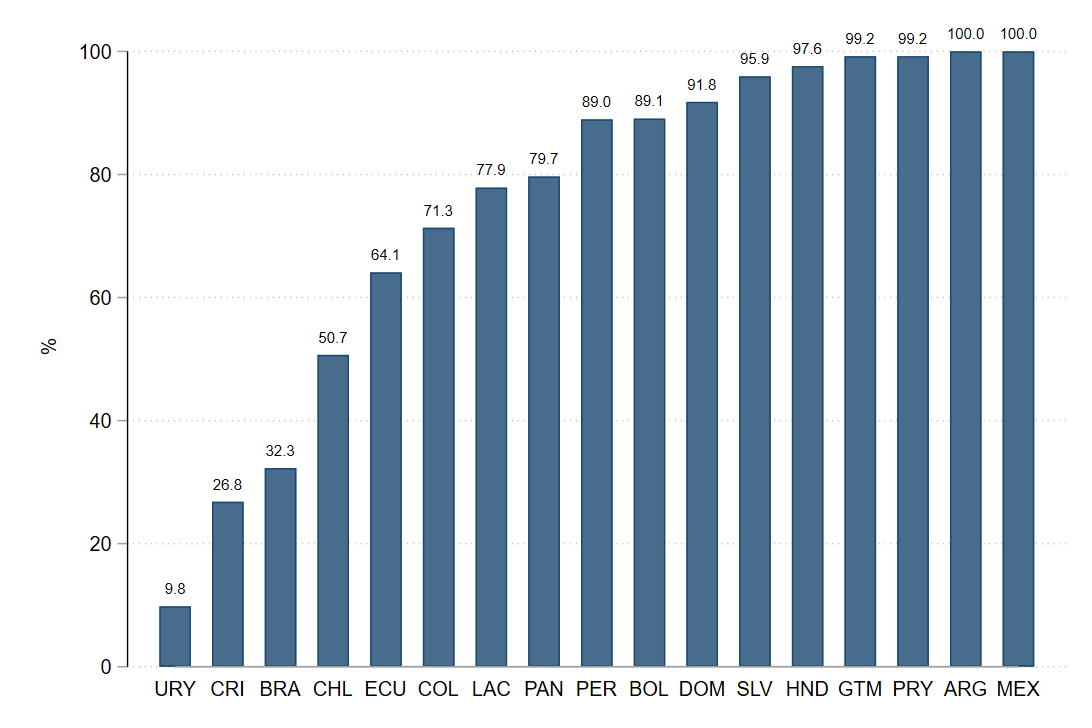
\includegraphics[scale=.3]{latex/figures/Self-employed/i_empgrowthfirm.png}}
                \label{fig:owner-}
                \footnotesize{Source: SEDLAC}
\end{figure}

\begin{figure}[H]
            \justifying
                \caption{Share of self-employed (independents and employers) who work in small firms and does not contributes to SS}  
            \centerline{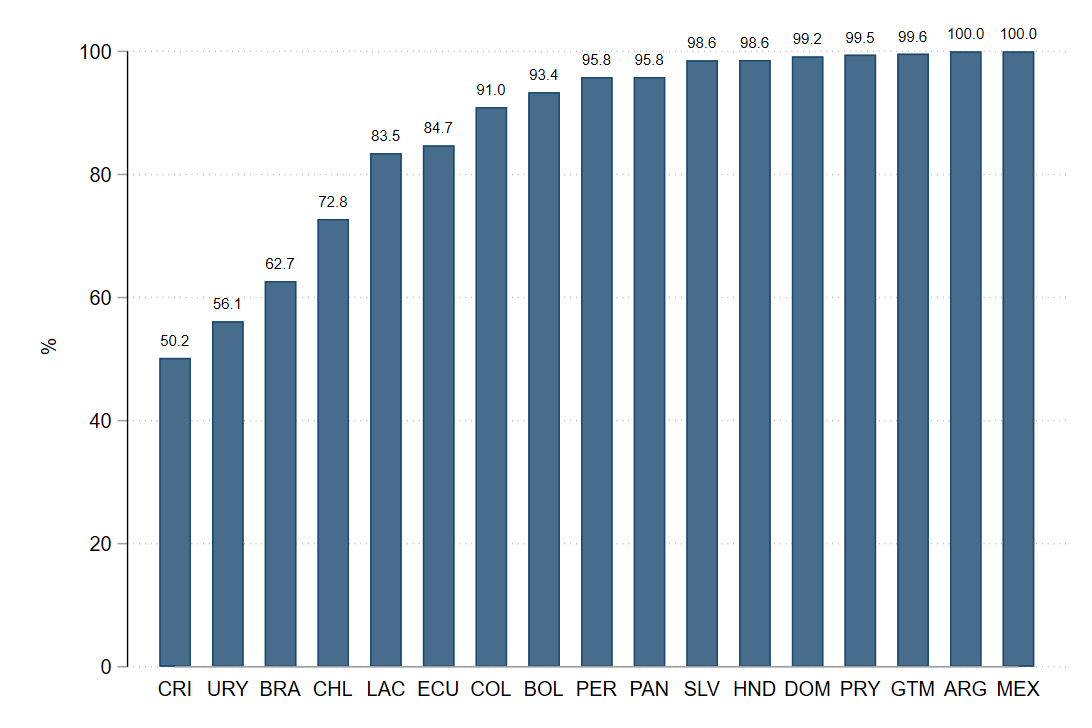
\includegraphics[scale=.3]{latex/figures/Self-employed/i_selfsmall.png}}
                \label{fig:owner-}
                \footnotesize{Source: SEDLAC}
\end{figure}

\begin{figure}[H]
            \justifying
                \caption{Share of self-employed (without employers) who does not contributes to SS: independent contractor}  
            \centerline{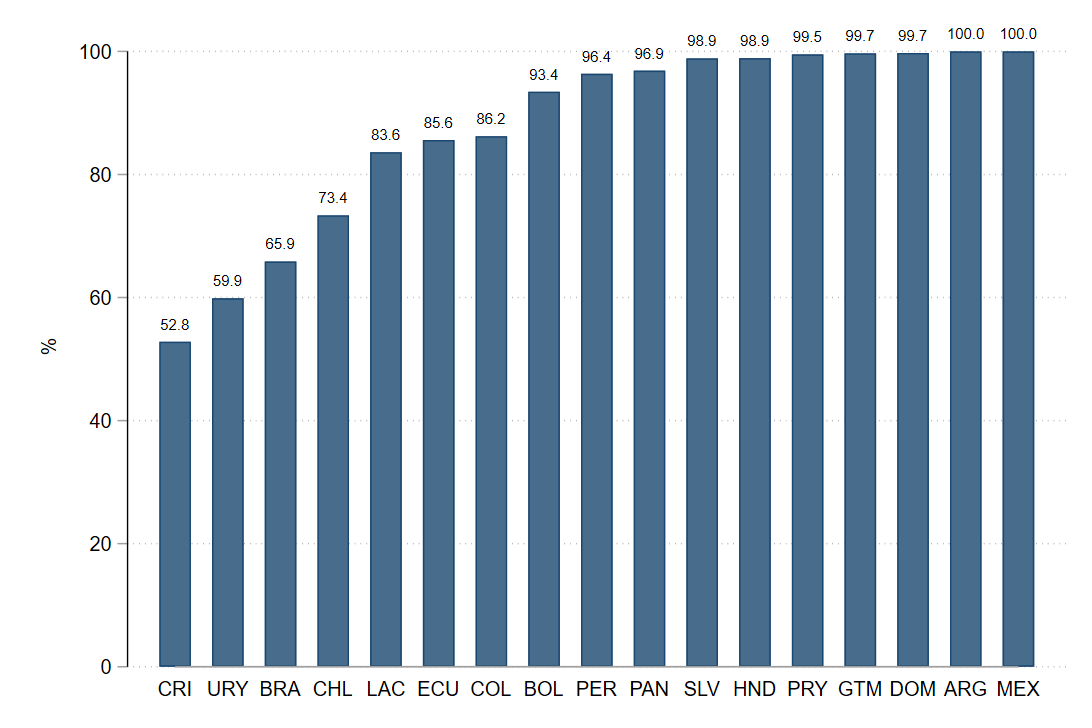
\includegraphics[scale=.3]{latex/figures/Self-employed/i_independent.png}}
                \label{fig:owner-}
                \footnotesize{Source: SEDLAC}
\end{figure}

\section{Family decision not worker decision}

\begin{figure}[H]
            \justifying
                \caption{Share of not salaried workers in small firms}  
            \centerline{\includegraphics[scale=.3]{latex/figures/Self-employed/n.png}}
                \label{fig:owner-}
                \footnotesize{Source: SEDLAC}
\end{figure}

\begin{figure}[H]
            \justifying
                \caption{Share of self-employed (independents and employers) who work in small firms and does not contributes to SS}  
            \centerline{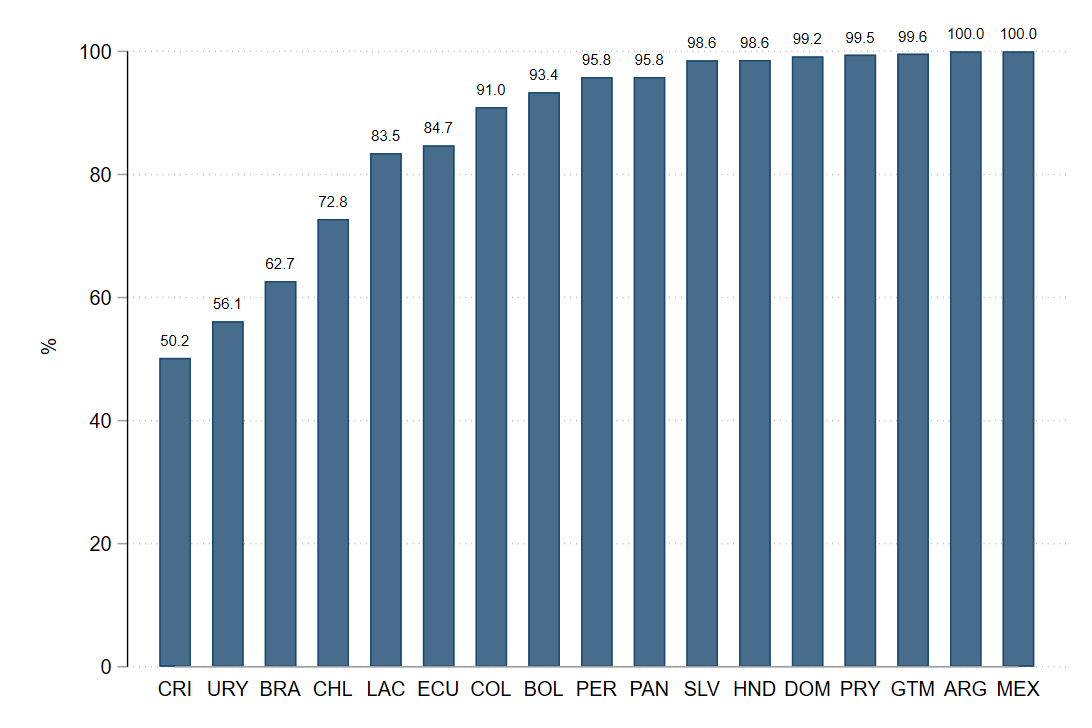
\includegraphics[scale=.3]{latex/figures/Self-employed/i_selfsmall.png}}
                \label{fig:owner-}
                \footnotesize{Source: SEDLAC}
\end{figure}

\begin{figure}[H]
            \justifying
                \caption{Share of self-employed (without employers) who does not contributes to SS: independent contractor}  
            \centerline{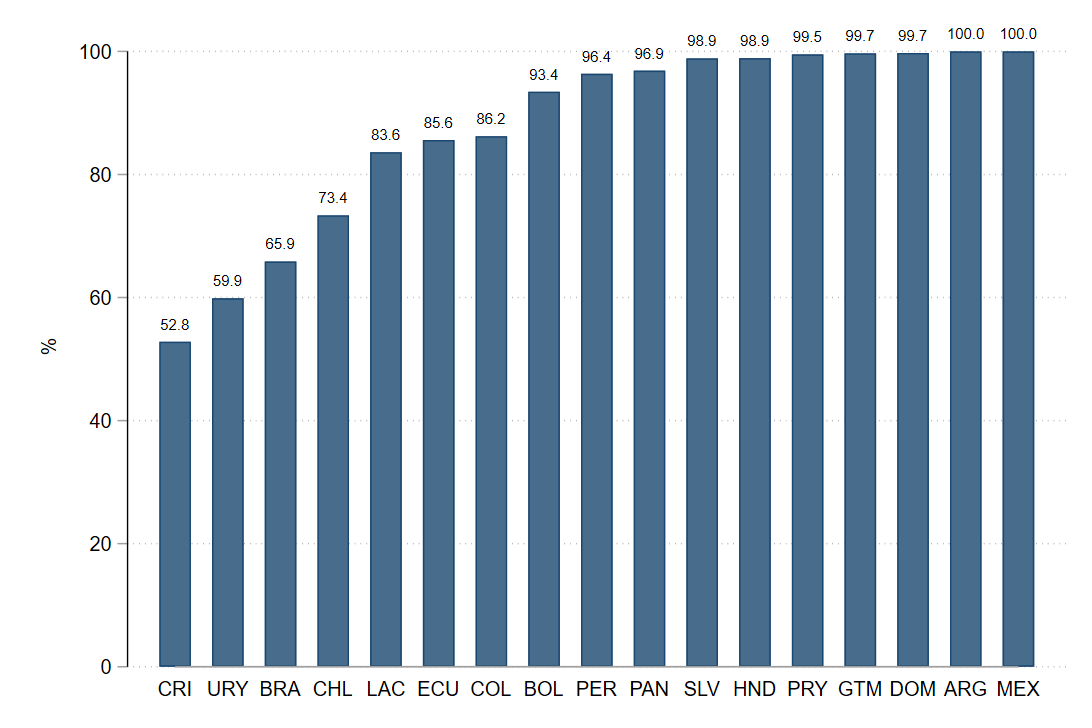
\includegraphics[scale=.3]{latex/figures/Self-employed/i_independent.png}}
                \label{fig:owner-}
                \footnotesize{Source: SEDLAC}
\end{figure}


\end{document}

